\documentclass[10pt]{beamer}


% Setup appearance:

\usetheme{TALK}
\usefonttheme[onlylarge]{structurebold}
\setbeamerfont*{frametitle}{size=\normalsize,series=\bfseries}
\setbeamertemplate{navigation symbols}{}

%\usecolortheme{seahorse}
%\usecolortheme{beaver}
%\usecolortheme{beetle}
%\usecolortheme{dolphin}
%\usecolortheme{dove}
%\usecolortheme{sidebartab}
%\usecolortheme{wolverine}



% Standard packages

\usepackage[english]{babel}
\usepackage[latin1]{inputenc}
\usepackage{times}
\usepackage[T1]{fontenc}
\usepackage{listings}



% Setup TikZ

\usepackage{tikz}
\usetikzlibrary{arrows}
\tikzstyle{block}=[draw opacity=0.7,line width=1.4cm]

% Setup Listings
%\lstset{backgroundcolor=\color{lightgray},basicstyle=\footnotesize,language=java}
\lstset{tabsize=2,basicstyle=\scriptsize\rmfamily,language=java,frameround=fttt,frame=trBL}


\setbeamercovered{transparent}

% Author, Title, etc.

\title[Service-Varianten und zustandsbehaftete Services auf Basis von OSGi] 
{%
  Realisierung von Service-Varianten\\und zustandsbehafteten Services\\ auf Basis von OSGi
}

% \subtitle{
% 	Erfahrungsbericht �ber den Einsatz von OSGi als Plattform f�r die Entwicklung von ``SiDiff''
% }

\author[Timo Kehrer]
{
  \underline{Timo Kehrer} \and
  Sven Wenzel \and
  Maik Schmidt
}

\institute[Universit�t Siegen]
{
%Dept. of Computer Science and Media \\
%Stuttgart Media University (HdM) \\
%Nobelstr. 10, D-70569 Stuttgart, Germany \\
%kehrer@mi.hdm-stuttgart.de\inst{1} \\
%ihler@hdm-stuttgart.de\inst{2} \\

Universit�t Siegen, Praktische Informatik\\
\{kehrer, wenzel, mschmidt\}@informatik.uni-siegen.de\\
\hfill\\
}

\date[OSGi 2009]
{OSGi Users'-Forum Treffen 2009\\27.10.2009 @ Eclipse Summit in Ludwigsburg}



% The main document

\begin{document}


\begin{frame}
  \titlepage
\end{frame}

\begin{frame}{Outline}
  \tableofcontents
\end{frame}


\section{OSGi-Einsatzkontext: ``SiDiff''}
\begin{frame}{Outline}
  \tableofcontents[current]
\end{frame}

\subsection{Applikationsdom�ne}

\begin{frame}{Versionen und Varianten technischer Dokumente}
	\begin{itemize}
		\item Technische Dokumente mit grafischer Notation gewinnen zunehmend an Bedeutung, bspw.
		\begin{itemize}
			\item CAD-Dokumente
			\item UML-Modelle
			\item Matlab/Simulink-Modelle
			\item etc.
		\end{itemize}
		
		\medskip
		\pause
		\item Komplexe Dokumente werden in der Regel im Team bearbeitet und in Repositories gespeichert
		\item Dokumente existieren in mehreren Versionen (Revisionen oder Varianten)
		\item Daraus resultieren eine Reihe praktischer Probleme:
		\begin{itemize}
			\item Konfigurationsmanagement (Diff/Merge)
			\item Analyse von Dokumenthistorien
			\item Clone Detection
			\item etc.
		\end{itemize}
	\end{itemize}
\end{frame}

\subsection{Problemmotivation}

\begin{frame}{Textuelle Dokumente vs. grafische/graphbasierte Dokumente}
	\begin{center}
		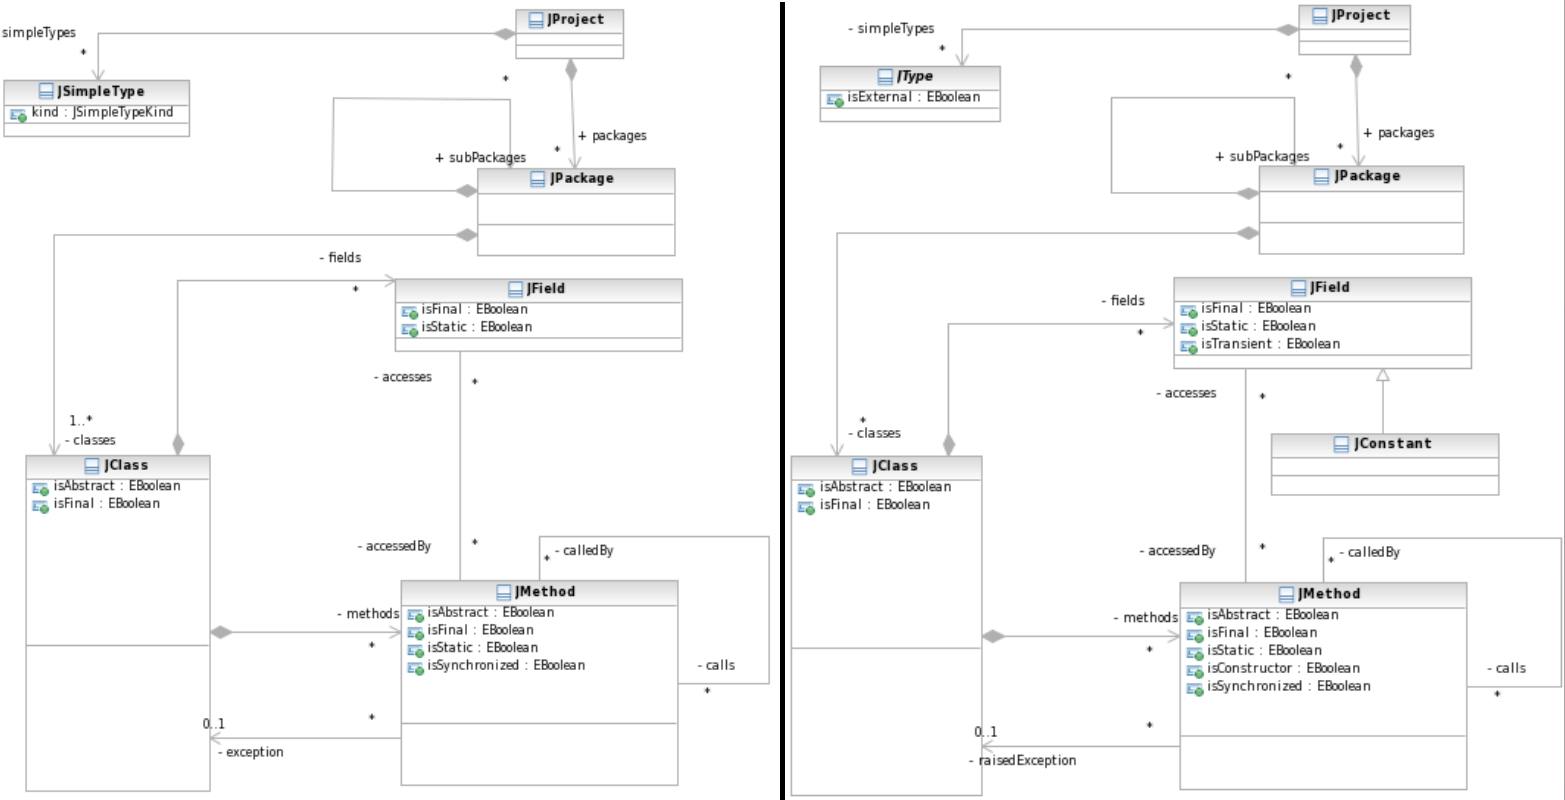
\includegraphics[scale=0.27]{graphics/wo-diff} 
	\end{center}
\end{frame}

\begin{frame}{Differenzen auf Basis der textuellen Repr�sentation}
	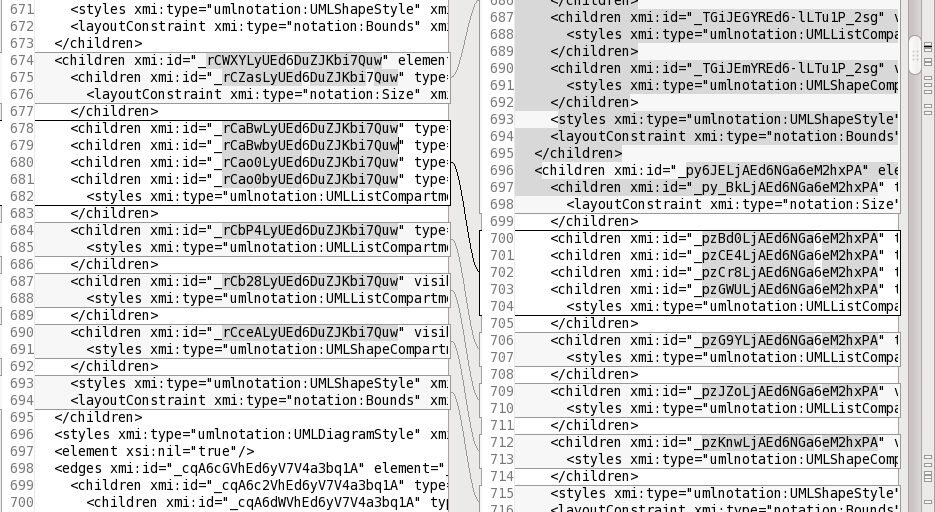
\includegraphics[scale=0.40]{graphics/text-diff}\\
	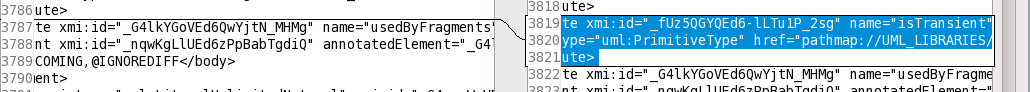
\includegraphics[scale=0.37]{graphics/text-diff-1}\\
	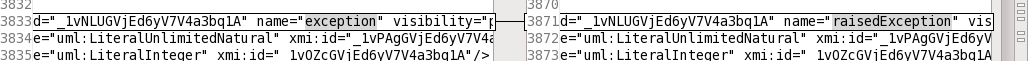
\includegraphics[scale=0.37]{graphics/text-diff-2}\\	
\end{frame}

\begin{frame}{Konzeptuelle Differenzen}
	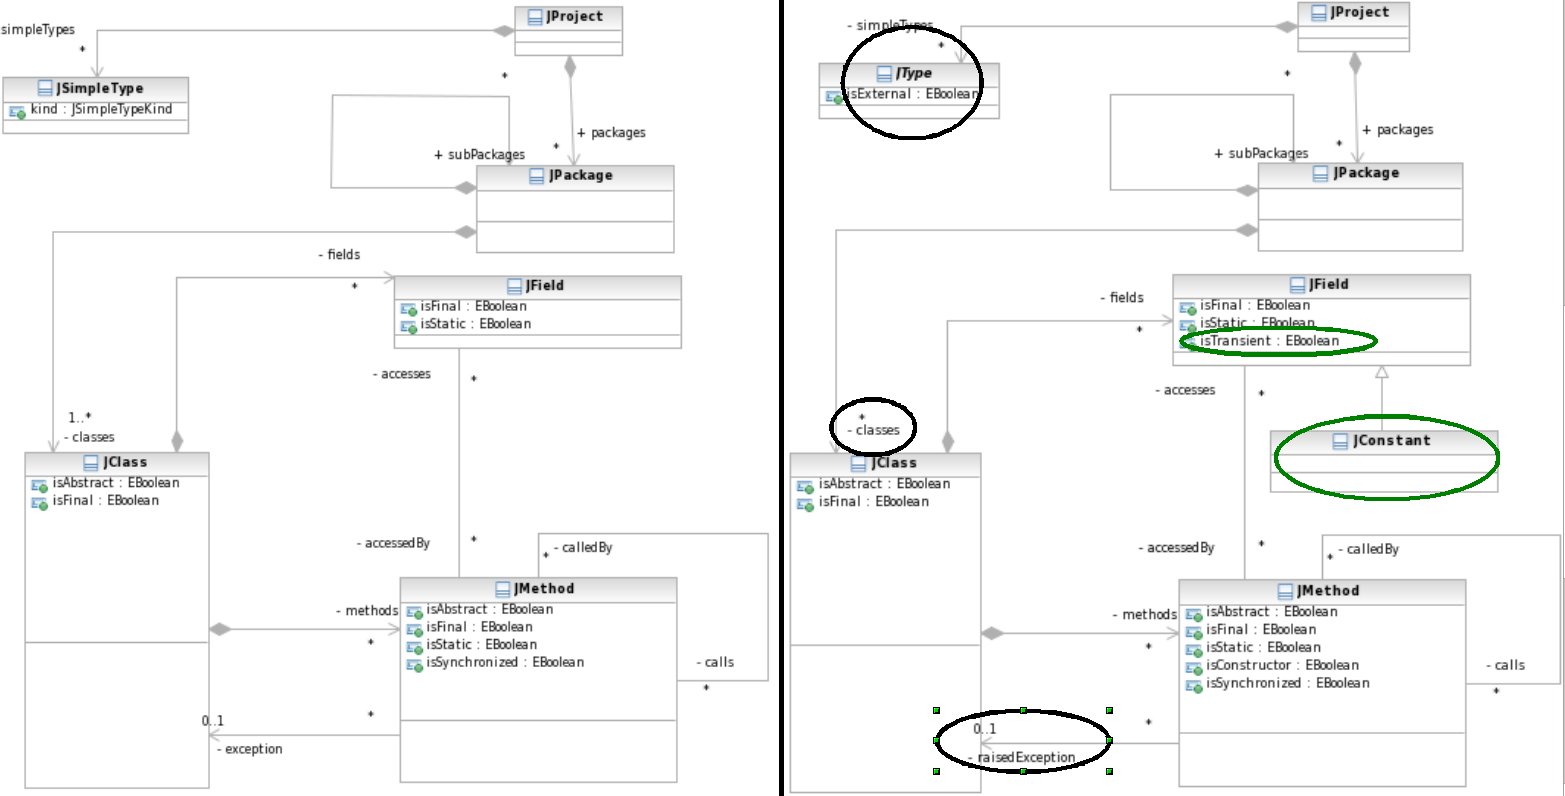
\includegraphics[scale=0.27]{graphics/see-diff}\\
\end{frame}

\begin{frame}{Fazit}
	\begin{itemize}
		\item Text-orientierte Werkzeuge ungeeignet f�r technische Dokumente mit grafischer Notation
		\medskip
		\item Einsatz grafischer Dokumente und Modelle rasant zunhemend, bspw. im Zuge moderner Entwicklungsparadigmen wie der modellbasierten Software-Entwicklung (MDA, MDD, MDSD, etc.)
		\medskip
		\item Daher Bedarf f�r hoch optimierte Verfahren und Werkzeuge f�r Modelle und grafische Dokumente
		\medskip
		\item $\rightarrow$ \textbf{SiDiff-Projekt} (\url{www.sidiff.org})
	\end{itemize}
\end{frame}


\section{Warum OSGi?}
\begin{frame}{Outline}
  \tableofcontents[current]
\end{frame}

\subsection{Architektur}

\begin{frame}{Workflow (Hier: Diff-Prozess)}
	\begin{center}
		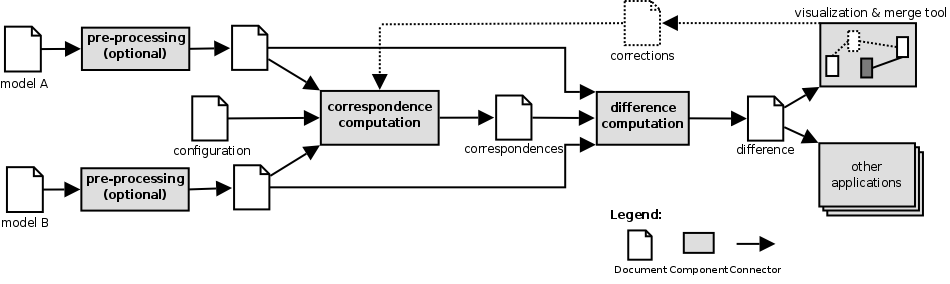
\includegraphics[scale=0.22]{graphics/compareprocess}
	\end{center}
\end{frame}

\begin{frame}{Komponenten und Services (Hier: Diff-Applikation, vereinfacht)}
	\begin{center}
		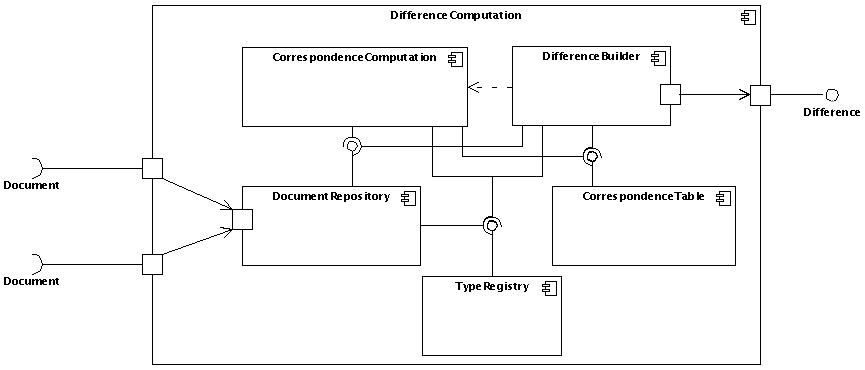
\includegraphics[scale=0.3]{graphics/diffcomponent}
	\end{center}
\end{frame}


\subsection{Technologische Umsetzung}

\begin{frame}{Gr�nde f�r den Einsatz von OSGi}
	\begin{block}{Architektonische Gr�nde}
		\begin{itemize}
			\item Flexibilit�t, Austauschbarkeit
			\item Lose Kopplung von klar definierten Komponenten/Services
		\end{itemize}
	\end{block}
	
	\pause
	\begin{block}{Organisatorische Gr�nde}
		``Echtes'' Geheimhaltungsprinzip auf Komponentenebene:
		\begin{itemize}
			\item Einhaltung von Konventionen weitestgehend durch das Framework sichergestellt
			\item Effektive Ma�nahme um der Degeneration der Architektur entgegen zu wirken 
		\end{itemize}
	\end{block}
			
	\pause
	\begin{block}{Pragmatische Gr�nde}
		\begin{itemize}
			\item Umsetzung des Service-Konzepts auf Basis von Java
			\item Nahtlose Integration in die Eclipse IDE
		\end{itemize}
	\end{block}
\end{frame}


\section{Realisierungs-Probleme}
\begin{frame}{Outline}
  \tableofcontents[current]
\end{frame}

\subsection{Einf�hrendes Beispiel}

\begin{frame}{3-Wege-Vergleich/-Mischen}
	\begin{center}
		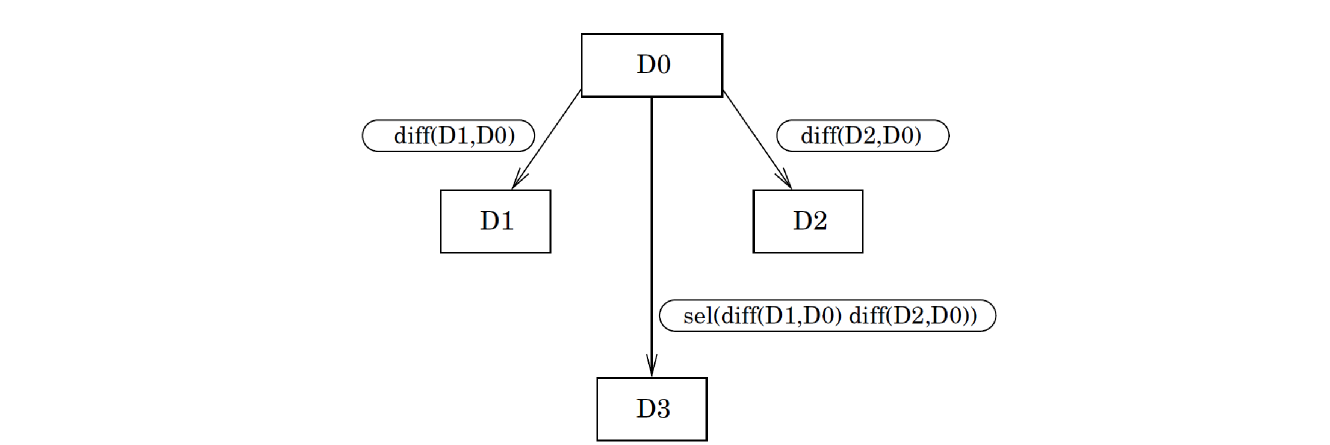
\includegraphics[scale=0.3]{graphics/3-way-1}
	\end{center}
\end{frame}
\begin{frame}{3-Wege-Vergleich/-Mischen}
	\begin{center}
		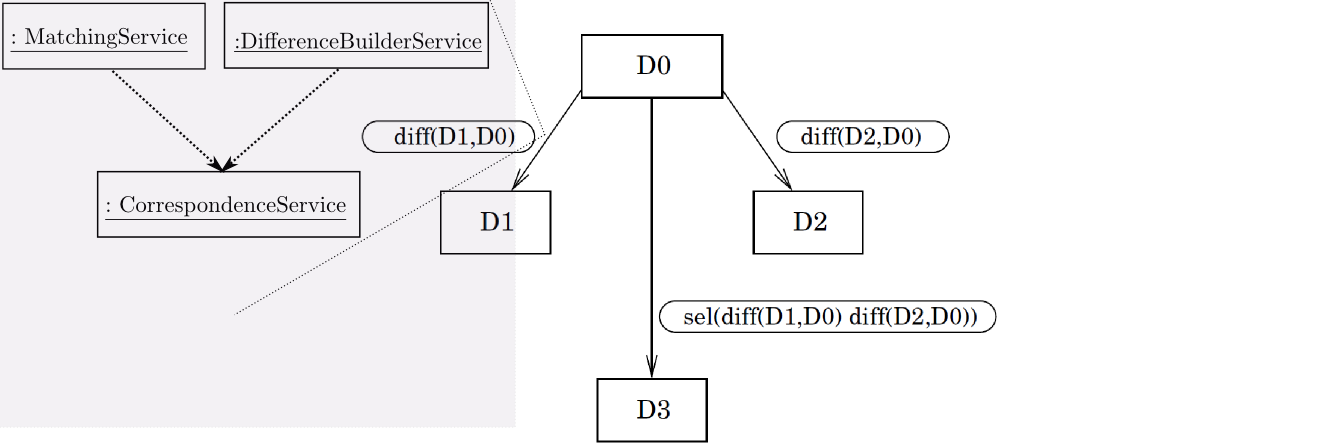
\includegraphics[scale=0.3]{graphics/3-way-2}
	\end{center}
\end{frame}
\begin{frame}{3-Wege-Vergleich/-Mischen}
	\begin{center}
		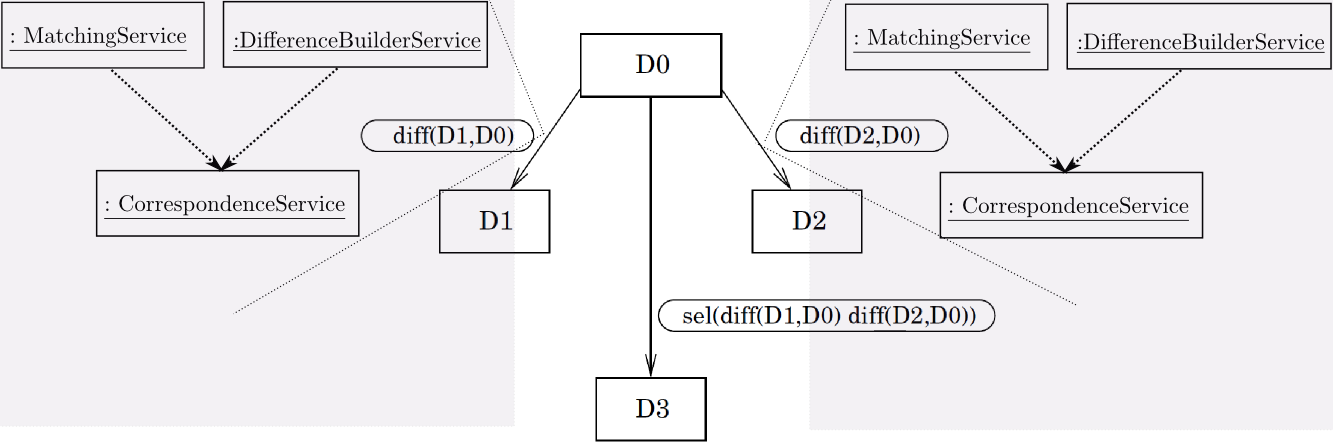
\includegraphics[scale=0.3]{graphics/3-way-3}
	\end{center}
\end{frame}



\subsection{Zustandsbehaftete Services}

\begin{frame}{Nutzung von Services in verschiedenen Kontexten}
	\begin{itemize}
		\item Es kann oft vorkommen, dass ein Service gleichzeitig in verschiedenen Kontexten genutzt werden soll.
		\medskip
		\item Problematisch ist dies f�r zustandsbehaftete Services
		\medskip
		\item Hier kann nicht genau eine Service-Instanz beim OSGi-Framework registriert werden.
		\bigskip
		\item Ein erster L�sungsansatz ist die OSGi Service Factory
	\end{itemize}
\end{frame}

\begin{frame}{Die OSGi Service Factory und deren Grenzen}
	\begin{block}{OSGi Service Factory}
		\begin{itemize}
			\item Die Service Factory ist Bestandteil des OSGi Standards.
			\item Kann anstatt des eigentlichen Services beim OSGi-Framework registriert werden.
			\item Die eigentliche Service-Instanz wird bei der Anforderung des Services transparent
				�ber die Factory erzeugt.
		\end{itemize}
	\end{block}	
	
	\pause
	\begin{block}{Grenzen der OSGi Service Factory}
		\begin{itemize}
			\item Die erzeugten Service-Instanzen werden vom OSGi-Framework \textbf{pro anfragendem Bundle} gecached.
			\item Szenarien, in denen ein Bundle verschiedene Instanzen eines Services erhalten sollen sind damit nicht realisierbar.
		\end{itemize}
	\end{block}
\end{frame}



\subsection{Service-Varianten}


\begin{frame}{Konfigurierbare Services und Service-Varianten}
	\begin{itemize}
		\item Oftmals ben�tigen wir Services, die z.B. f�r einen bestimmten Dokumenttyp konfiguriert werden.
		\begin{itemize}
			\item Ein Beispiel ist der �hnlichkeits-basierte Matching-Service, welcher durch eine Dokumenttyp-spezifische Heuristik konfiguriert wird. 
		\end{itemize}
		
		\medskip
		\pause
		\item Zudem sollte die Koexistenz von mehreren Service-Instanzen, welche verschieden konfiguriert sind unterst�tzt werden.
		\begin{itemize}
			\item So zum Beispiel beim Einsatz von SiDiff im Rahmen einer Entwicklungsumgebung, welche mehrere Dokumentypen unterst�tzt.
		\end{itemize}
	\end{itemize}
\end{frame}


\section{L�sungsans�tze und technische Umsetzung}
\begin{frame}{Outline}
  \tableofcontents[current]
\end{frame}

\subsection{Kapselung der OSGi Service-Schicht}
\begin{frame}{Outline}
  \tableofcontents[current, currentsubsection]
\end{frame}

\begin{frame}{Der Service-Helper}
	\begin{columns}[onlytextwidth]
		\column{.6\textwidth}
		\begin{itemize}
			\item Keine direkte Kommunikation mit dem OSGi-Framework �ber den OSGi-BundleContext
			\item Service-Helper kapselt die Zugriffe auf den Service-Layer des OSGi-Frameworks
			\item Allgemeine Schnittstelle f�r Aufgaben wie bspw. die Registrierung oder das Anfordern von Services
		\end{itemize}
		\column{.4\textwidth}
		\vfill
		\begin{center}
		  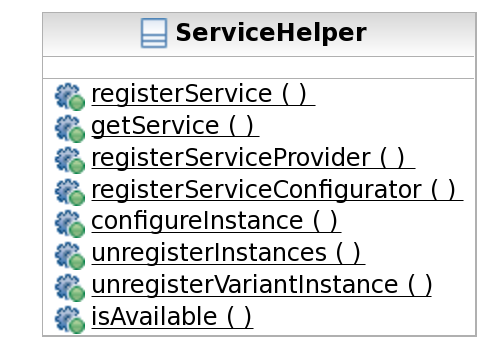
\includegraphics[width=\textwidth]{graphics/service-helper}\\
		\end{center}
		\vfill
	\end{columns} 
\end{frame}




\subsection{Zustandsbehaftete Services: ``ProvideableService''}
\begin{frame}{Outline}
  \tableofcontents[current, currentsubsection]
\end{frame}

\begin{frame}{Definition der Service-Schnittstelle}
	\begin{center}
		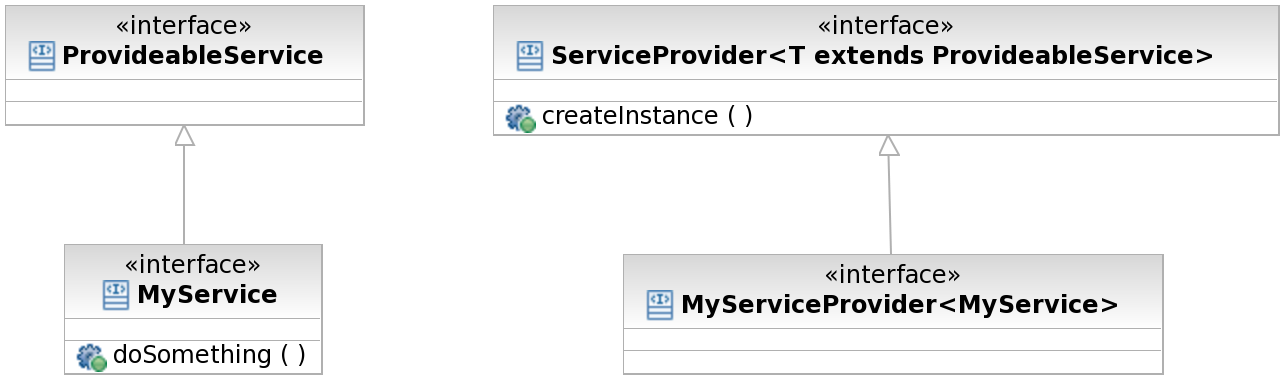
\includegraphics[scale=0.3]{graphics/provideable-interface.png}
	\end{center}

	\begin{columns}[onlytextwidth]
		\column{.35\textwidth}
		\begin{itemize}
			\item ``Leeres'' Interface 
			\item Dient als ``Marker'' im automatischen Instanziierungsprozess
		\end{itemize}
		\vfill
		
		\column{.65\textwidth}
		\begin{itemize}
			\item Hei�t wie die Service-Schnittstelle tr�gt das Suffix \texttt{Provider}.
			\item Liegt im selben Paket wie die Service-Schnittstelle.
			\item Erbt vom Interface \texttt{ServiceProvider}, getypt auf die Service-Schnittstelle.
		\end{itemize}
 	\end{columns}
\end{frame}

\begin{frame}{Implementierung des Services}
	\begin{center}
		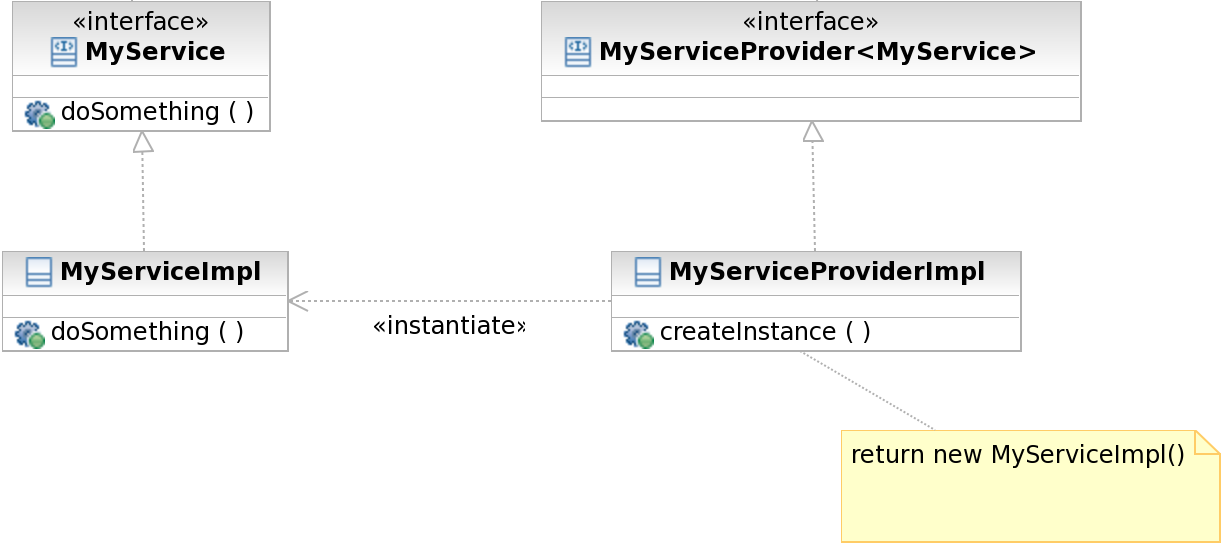
\includegraphics[scale=0.3]{graphics/provideable-impl.png}
	\end{center}
	\vspace{0.5cm}
	
	\begin{columns}[onlytextwidth]
		\column{.4\textwidth}
		\begin{itemize}
			\item Implementierung des Dienstes
		\end{itemize}
		
		\column{.6\textwidth}
		\begin{itemize}
			\item Erzeugung einer Instanz des Dienstes
		\end{itemize}
 	\end{columns}
	
\end{frame}


\begin{frame}[containsverbatim]
	\frametitle{Bekanntmachen der Service-Implementierung}
\begin{lstlisting}
public class Activator implements BundleActivator {

	public void start(BundleContext context) throws Exception {
		ServiceHelper.registerServiceProvider(
			context,
			MyServiceProvider.class,
			new MyServiceProviderImpl(),
			null,											// DocType
			null);										// Variant
	}

	public void stop(BundleContext context) throws Exception {
	}

}
\end{lstlisting}
\vspace{0.05cm}

\begin{itemize}
	\item Registriert wird der \texttt{ServiceProvider}
	\item Die Service-Implementierung selbst muss nicht registriert werden
	\item Sie wird �ber den \texttt{ServiceProvider} bereitgestellt
\end{itemize}
\end{frame}


\begin{frame}[containsverbatim]
	\frametitle{Verwenden des Services}
\begin{lstlisting}
MyService ms = ServiceHelper.getService(
				context, 					\\BundleContext
				MyService.class, 	\\ServiceInterface
				null, 						\\ DocumentType
				null);						\\ Variant
ms.doSomething();	
\end{lstlisting}
\vspace{0.5cm}

\begin{itemize}
	\item Der Zugriff auf den Provider und die Instanzierung der eigentlichen Service-Implementierung erfolgt transparent.
	\bigskip
	\item Der \texttt{ServiceHelper} pr�ft, ob der angeforderte Service ein \texttt{ProvideableService} ist. 
	\item Wenn ja, wird beim OSGi-Framework ein entsprechend benannter \texttt{ServiceProvider} (hier \texttt{MyServiceProvider}) gesucht und dessen \texttt{createInstance()}-Methode aufgerufen.
\end{itemize}
\end{frame}


\subsection{Service-Varianten: ``ConfigurableService''}
\begin{frame}{Outline}
  \tableofcontents[current, currentsubsection]
\end{frame}

\begin{frame}[containsverbatim]
	\frametitle{Definition der Service-Schnittstelle}
\begin{itemize}
	\item Konfigurierbare Services m�ssen das Interface \texttt{ConfigurableService} erweitern.
\end{itemize}
\vspace{0.2cm}
\begin{lstlisting}
public interface ConfigurableService {
	public String configure(Object... configData);
	public void deconfigure();
	public Dictionary<String, String> getProperties();
}
\end{lstlisting}
\vspace{0.2cm}	
	
\begin{itemize}	
	\item Die \texttt{configure()}-Methode wird aufgerufen, um den Service mit beliebigen Daten (\texttt{Object...}) zu konfigurieren.
	\item Der R�ckgabewert der \texttt{configure()}-Methode ist der Dokumenttyp f�r den die Konfiguration geeignet ist.\\
		Da sich der Typ i.d.R. aus den Konfigurationsdaten ableitet, kann er sinnvollerweise nur hier ermittelt werden.
\end{itemize}
\end{frame}

\begin{frame}[containsverbatim]
	\frametitle{Implementierung des Services}
\begin{itemize}
	\item Implementierung unterscheidet sich von ``einfachen Services'' nur durch die zus�tzlichen Methoden des \texttt{ConfigurableService}
 	\item damit wird der Service-Instanz die Konfiguration �bergeben
�bergeben wird.
\end{itemize}
\vspace{0.1cm}
\begin{lstlisting}
public class MyConfigurableServiceImpl implements MyConfigurableService	

	String docType;
	
	public String configure(Object... configData) {
		// ...
		return docType;
	}

	public void deconfigure() {
	}

	public Dictionary<String, String> getProperties() {
		return null;
	}
}
\end{lstlisting}

\end{frame}

\begin{frame}[containsverbatim]
	\frametitle{Bekanntmachen der Service-Implementierung}

\begin{itemize}
	\item Registrierung der Schnittstelle und der konkreten Implementierung des konfigurierbaren Services beim \texttt{ServiceHelper}
\end{itemize}
\vspace{0.4cm}

\begin{lstlisting}
public class Activator implements BundleActivator {

	public void start(BundleContext context) throws Exception {
		ServiceHelper.registerServiceConfigurator(
					context, 
					MyConfigurableService.class, 
					MyConfigurableServiceImpl.class);
	}
	
	public void stop(BundleContext context) throws Exception {
	}

}
\end{lstlisting}	
\end{frame}


\begin{frame}[containsverbatim]
	\frametitle{Konfiguration des Services}

	\begin{columns}[onlytextwidth]
		\column{.5\textwidth}
		
Methode des ServiceHelpers:
\begin{lstlisting}
public static void configureInstance(
	BundleContext context,
	Class<?> interfaceClass,
	String docType,
	String variant,
	Object... configData)
\end{lstlisting}

		\column{.45\textwidth}
		
Aufrufbeispiel:
\begin{lstlisting}
ServiceHelper.configureInstance(
	context,
	MyConfigurableService.class,
	getEPackage().getNsURI(),
	"SIMPLE", 
    "config.xml");
\end{lstlisting}
	
	\end{columns}

\vspace{0.4cm}
\begin{itemize}
 	\item Anschlie�end steht der Service in konfigurierter Form zur Verf�gung.
 	\medskip
 	\item Die eigentliche Konfiguration erfolgt transparent durch den \texttt{ServiceHelper}.
\end{itemize}

\end{frame}


\begin{frame}[containsverbatim]
	\frametitle{Verwenden des Services}
\begin{itemize}
	\item Um einen fertig konfigurierten Service zu verwenden, wird dieser wie alle anderen Services �ber den \texttt{ServiceHelper} angefordert.
	\medskip
	\item Hier m�ssen jedoch der Dokumenttyp oder der Dokumenttyp und die Variante als Parameter mitgegeben werden, z.B.: 
\end{itemize}

\vspace{0.3cm}
\begin{lstlisting}
MyService ms = ServiceHelper.getService(
				context, 
				MyConfigurableService.class,
				eObj.eClass().getEPackage().getNsURI(),
				"SIMPLE");
\end{lstlisting}
\end{frame}


\subsection{Kombination: ``ConfigurableProvideableService''}
\begin{frame}{Outline}
  \tableofcontents[current, currentsubsection]
\end{frame}

\begin{frame}{Konfigurierbare und zustandsbehaftete Services}
	\begin{center}
		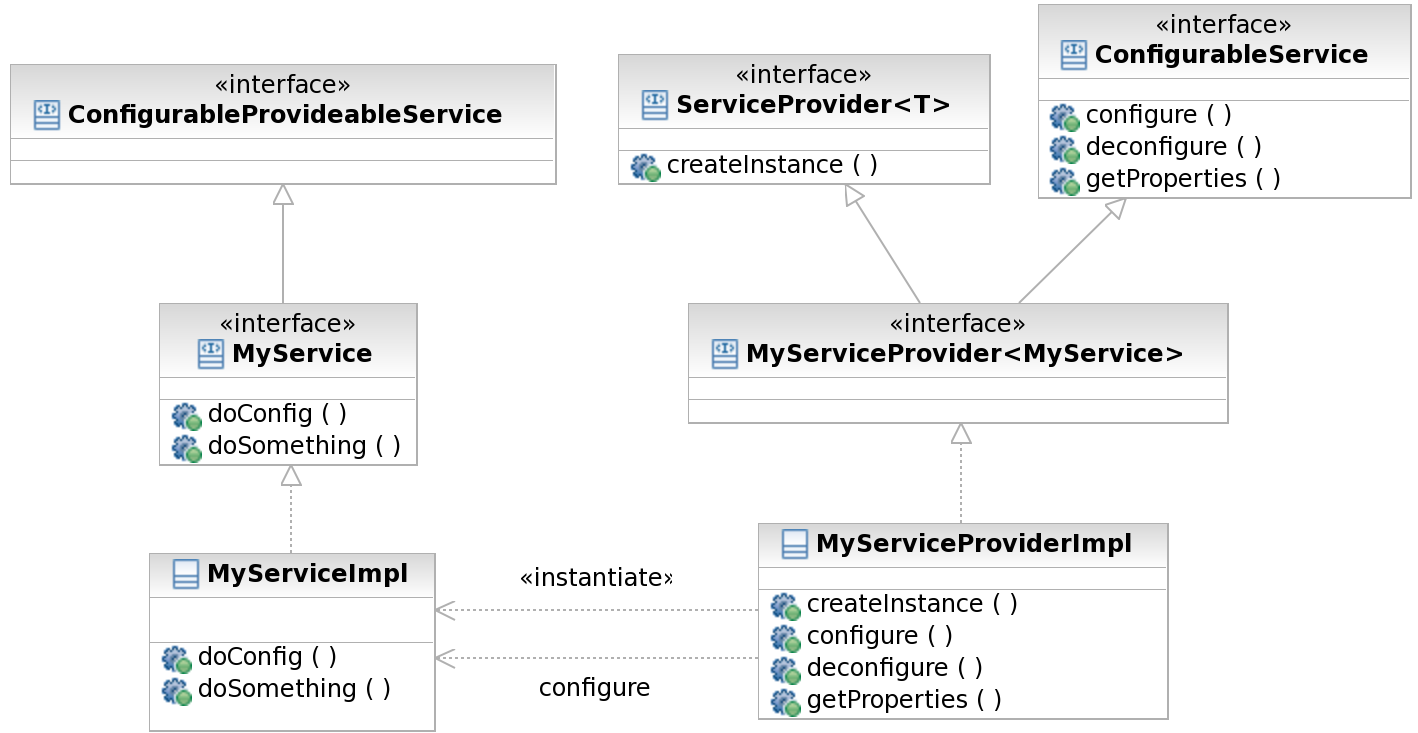
\includegraphics[scale=0.3]{graphics/provideable-configurable.png}
	\end{center}
\end{frame}


\section*{Zusammenfassung}


\begin{frame}{Zusammenfassung}
	\begin{itemize}
		\item SiDiff als Werkzeugkasten zum Bau von Differenz- und Mischwerkzeugen f�r Modelle
		\item Realisierung einer Service-orientierten Architektur auf Basis von OSGi
		\medskip
		\item Umsetzung der SiDiff-spezifischen Anforderungen durch eine auf dem OSGi Standard aufbauende Service-Schicht
		\begin{itemize}
			\item Kapselung des OSGi-Frameworks
			\item Unterst�tzung von zustandsbehafteten Services
			\item Unterst�tzung von Service-Varianten
			\item Unterst�tzung der Kombination beider Service-Arten
		\end{itemize}
	\end{itemize}

\end{frame}



\begin{frame}{Vielen Dank f�r Ihre Aufmerksamkeit}
	\vspace{1cm}
	\begin{center}
		\Large Fragen?
	\end{center}
	\normalsize
	\vspace{1cm}
	\begin{flushright}
 	
\includegraphics[scale=0.3]{graphics/sidiff.jpg}\\
	% sidiff.jpg: 200x115 pixel, 72dpi, 7.06x4.06 cm, bb=0 0 200 115
	\vspace{0.3cm}
	\url{www.sidiff.org}
	\end{flushright}

\end{frame}

\end{document}


